\documentclass{article}

\def\sectionnumber{7}
\def\sectiontitle{Covariance and Correlation, Multinomial, Multivariate Normal}

\usepackage{common}

% Set this false to hide, true to show
\setboolean{showanswers}{true}

\begin{document} 

\header

\section{Covariance and Correlation}

\begin{description}

\item[Covariance] $\cov(X, Y) = E[(X - EX)(Y - EY)] = E(XY) - E(X)E(Y)$. The covariance of independent r.v.s is 0, but if two r.v.s have covariance 0, they aren't necessarily independent.

\item[Key properties of covariance]

    \begin{enumerate}
        \item $\cov(X, X) = \var(X)$
        
        \item $\cov(X, Y) = \cov(Y, X)$
        
        \item $\cov(X, c) = \cov(c, X) = 0$ for any constant $c$
        
        \item $\cov(aX, Y) = a\cov(X, Y)$ for any constant $a$
        
        \item $\cov(X + Z, Y) = \cov(X, Y) + \cov(Z, Y)$ -- covariance is distributive (very similar to multiplication)
        
        \item $\var(X_1 + \dots + X_n) = \var(X_1) + \dots + \var(X_n) + 2\sum_{i < j} \cov(X_i, X_j)$
    \end{enumerate}

\item[Correlation] $\corr(X, Y) = \frac{\cov(X, Y)}{\SD(X)\SD(Y)}$. Correlation $\rho$ always satisfies $-1 \leq \rho \leq 1$. Note that independent variables always have correlation zero, but the converse is not generally true (unless you're working with a multivariate normal, discussed below)

\end{description}

1. Mark is thinking about constructing a portfolio of two stocks: A and B. Suppose the annual percentage return $R_A$ of stock A is distributed as $\N(\mu=10, \sigma^2=25)$, while those of stock B (call it $R_B$) are distributed as $\N(\mu=5, \sigma^2=9)$. Suppose $\corr(R_A,R_B) = -0.5$. For every share of stock $A$ in Mark's portfolio, how many shares of stock $B$ should he buy to minimize the variance of his portfolio's returns?

\hide{ Say Mark buys $b$ shares of stock $B$ per share of stock $A$. Then Mark's portfolio return per share of stock $A$ is given by $R \equiv R_A + bR_B$. We compute
\begin{align*}
    \var(R) & = \var(R_A+bR_B) \\
    & = \cov(R_A+bR_B,R_A+bR_B) \\
    & = \var(R_A) + 2b\cov(R_A,R_B) + b^2\var(R_B) \\
    & = 25 - 15b + 9b^2
\end{align*}
where we've computed $\cov(R_A,R_B) = \corr(R_A,R_B) \cdot \SD(R_A)\SD(R_B) = -7.5$. This expression is minimized when $b = \frac{15}{18} = \boxed{\frac{5}{6}}$.} 

2. (William Chen and Sebastian Chiu, 2013). For Christmas, $n$ people are doing a Secret Santa, where each person puts his or her name on a piece of paper in a hat and randomly picks a name from the hat without replacement. In this game, there is a possibility that people can select their own names and have to buy themselves a gift. :( 

\begin{figure}[!ht]
\begin{center}
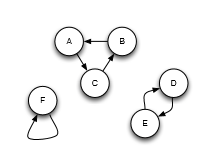
\includegraphics[width = 0.3\textwidth]{cycle.PNG}
\end{center}
\end{figure}

(a) What is the expected number of cycles that form? (Three examples of cycles are shown below.)

\hide{First we define the random variable of interest as $X$, where $X$ is the number of cycles that form. Next, we break up $X$ into its indicator random variables. We would like to count the number of cycles that happen on a person by person basis, so we split up $X$ into indicators that the $i$th person in Secret Santa completes a cycle after drawing a name from the hat. We have 
\[X = I_1 + I_2 + ... + I_n\]
We apply linearity of expected value and the fundamental bridge to express the expected value of $X$ in terms of the probabilities of each of the $n$ events:
\[E(X) = P(I_1=1) + P(I_2=1) + ... + P(I_n=1)\]
We note that $P(I_1 = 1/n)$: for the first person to choose, the only way that person will form a cycle is if that person chooses himself/herself. Continuing, $P(I_2 = 1/(n-1))$, as there are $n-1$ remaining choices in the hat, and only one of the draws will lead to a completed cycle (it could be the person himself/herself, or it could be the person who drew that person from the hat). The pattern continues until $P(I_n = 1)$ -- the last person who draws will always complete a cycle -- so
\[E(X) = \sum_{k=1}^n \frac{1}{k}\]
}


(b) What is the variance of the number of cycles that are formed? \\

\hide{Continuing from the previous question,
\[\var(X) = \var(I_1 + I_2 + ... + I_n) \]
and we can apply the properties of covariance as follows:
\begin{align*}
    \var(X) &= \cov(I_1 + I_2 + ... + I_n, I_1 + I_2 + ... + I_n) \\
    &= \cov(I_1, I_1) + \cov(I_2, I_2) + ... + \cov(I_n, I_n) + \sum_{i \neq j} \cov(I_i, I_j) \\
    &= \sum_{i=1}^n \var(I_i) + 2\sum_{i < j} \cov(I_i, I_j)
\end{align*}
Now note that $I_i$ and $I_j$ are independent, since knowing that $i$ forms a cycle does not affect the probability that $j$ forms a cycle; $E(I_i) = P(I_i = 1) = 1/(n-i+1)$ regardless of how many cycles have already been formed. The covariances therefore drop out, and we obtain
\begin{align*}
    \var(X) &= \sum_{i=1}^n \var(I_i) \\
    &= \sum_{i=1}^n \left( E(I_i^2) - [E(I_i)]^2 \right)\\
    &= \sum_{i=1}^n \left( E(I_i) - [E(I_i)]^2 \right) \\ 
    &= \sum_{i=1}^n \left( \frac{1}{i}\ -\left(\frac{1}{i}\right)^2 \right)\\ 
\end{align*}
}


\section{Multinomial}

\begin{description}

\item[Story] Each of $n$ objects is placed randomly and independently into $k$ categories. The probability of being placed into category $i$ is $p_i$. Let $\mathbf{p} = (p_1, p_2, \dots, p_k)$. Then the distribution of the number of objects in each category is $\Mult_k(n, \mathbf{p})$. This is a generalized version of the Binomial (the $j$th element of a $\Mult_k(n, \mathbf{p})$ random vector is distributed as a $\Bin(n, p_j)$).

\item[Joint PMF] $$P(X_1 = n_1, X_2 = n_2, \dots, X_k = n_k) = \frac{n!}{n_1!n_2!\cdots n_k!}p_1^{n_1}p_2^{n_2}\cdots p_k^{n_k}$$ You don't really have to remember this, but know that this is the generalization of the Binomial PMF.

\item[Lumping] If you lump more than one of the $k$ categories together, the result is still Multinomial. For example, lumping categories 1 and 2 together results in a Multinomial with new probability $p_1 + p_2$.

\end{description}

3. On July 4, 2012, the state of humanity's understanding of the universe took a large step forward with the discovery of the Higgs boson. Put simply, the way to discover the Higgs boson is to collide particles at high enough energies so that the boson is produced. Unfortunately, it decays extremely quickly into a bunch of elementary particles. For simplicity, let's suppose that a Higgs boson decays into one of three possible pairs: 1) fermion pair; 2) W boson pair; 3) Z boson pair. The events occur with probabilities $p$, $q$, and $1-p-q$, respectively. 

(a) What is the PMF of $F, W, Z$, signifying the number of times each of the decay events occur, given that we produce $n$ Higgs bosons?

\hide{$F, W, Z \sim \Mult_3(n, (p, q, 1 - p - q))$}

(b) What is the distribution of the number of fermion pair decays?

\hide{By lumping, we have: $F \sim \Bin(n, p)$.}

\section{Multivariate Normal}

\begin{description}

\item[Definition] A random vector is Multivariate Normal (MVN) if every linear combination of the elements is Normal.

\item[Uncorrelatedness and independence] Zero correlation between two elements of a MVN random vector implies that those two elements are independent. Keep in mind that this is \textit{only} true for Multivariate Normals.

\end{description}

4. Let $Z_1$ and $Z_2$ be independently standard normal. Prove that $Z_1+Z_2$ and $Z_1-Z_2$ are independent.

\hide{Notice that the vector $(Z_1+Z_2,Z_1-Z_2)$ is bivariate normal since any linear combination of the components takes the form $aZ_1+bZ_2$ which is normal (since sum of independent normals is normal). So it suffices to show that they are uncorrelated. But 
$$
    \cov(Z_1+Z_2,Z_1-Z_2) = \var(Z_1) - \cov(Z_1,Z_2) + \cov(Z_2,Z_1) - \var(Z_2) = 0
$$}

5. Let $Z$ be a standard normal random variable. Martha constructs a new standard normal random variable $W$ by flipping a fair coin and multiplying $Z$ by 1 if the coin lands heads and by -1 otherwise. Prove that $(W,Z)$ is NOT bivariate normal.

\hide{Since Normals are continuous, the probability that any Normal is 0 is 0. But $Z + W$ is $2Z$ half the time and $0$ otherwise, so there's a non-zero probability that $Z + W = 0$. Thus $Z + W$ isn't Normal, which means that $(W, Z)$ isn't MVN since all linear combinations of a MVN must be Normal.}

\end{document}

